%%%%%%%%%%%%%%%%%%%%%%%%%%%%%%%%%%%%%%%%%
% University/School Laboratory Report
% LaTeX Template
% Version 4.0 (March 21, 2022)
%
% This template originates from:
% https://www.LaTeXTemplates.com
%
% Authors:
% Vel (vel@latextemplates.com)
% Linux and Unix Users Group at Virginia Tech Wiki
%
% License:
% CC BY-NC-SA 4.0 (https://creativecommons.org/licenses/by-nc-sa/4.0/)
%
%%%%%%%%%%%%%%%%%%%%%%%%%%%%%%%%%%%%%%%%%

%----------------------------------------------------------------------------------------
%	PACKAGES AND DOCUMENT CONFIGURATIONS
%----------------------------------------------------------------------------------------

\documentclass[
	letterpaper, % Paper size, specify a4paper (A4) or letterpaper (US letter)
	10pt, % Default font size, specify 10pt, 11pt or 12pt
]{CSUniSchoolLabReport}

\usepackage{multirow}
\usepackage[backend=biber]{biblatex}
\usepackage{algorithm2e}
\usepackage[spanish]{babel}
\addbibresource{sample.bib} % Bibliography file (located in the same folder as the template)

%----------------------------------------------------------------------------------------
%	REPORT INFORMATION
%----------------------------------------------------------------------------------------

\title{Edge band width \\ Análisis y diseño de algoritmos} % Report title

\author{Luis Alberto \textsc{Ballado Aradias}} % Author name(s), add additional authors like: '\& James \textsc{Smith}'

\date{\today} % Date of the report

%----------------------------------------------------------------------------------------

\begin{document}

\maketitle % Insert the title, author and date using the information specified above

% If you need to include an abstract, uncomment the lines below
%\begin{abstract}
%	Abstract text
%\end{abstract}

%----------------------------------------------------------------------------------------
%	OBJECTIVE
%----------------------------------------------------------------------------------------

\section{Introducción}

El cálculo del edge bandwidth es una problematica importante en redes de comunicaciones para determinar la capacidad de transferencia de datos entre dos nodos en la red.\\

El max bandwidth se refiere a la cantidad máxima de datos que pueden transferirse por segundo a través de una conexión entre dos nodos de la red. El cálculo puede ser de gran utilidad en diferentes situaciones, una de ellas es para la optimizar la capacidad de transferencia de datos de una red, para así identificar los cuellos de botella en la red que puedan estar afectando el rendimiento, o para planificar la expansión de una infraestructura de red. Además, es de gran utilidad en aplicaciones de transmisión de video en tiempo real, la transferencia de archivos de gran tamaño solo por mencionar algunas.\\

Partiendo de ello, se busca crear una estructura de datos que nos ayude talvez no a comparar ni proponer nuevos tiempos, si no poder aplicar estructuras que nos ayude a hacer un análisis de manera eficiente sin repetir tanto nuestro código.\\

El cálculo del \textbf{edge-bandwidth} de un grafo es el mínimo entre todos los posibles costos de aristas de la máxima diferencia entre dos aritas adyacentes. 

\begin{center}
  \[B_f(G) = max{|f(u)-f(v)|: uv \in E}\]
\end{center}

\newpage
\section{Pseudocódigos}

\SetKwComment{Comment}{/* }{ */}

\begin{algorithm}
\caption{Evaluación Secuencial}\label{alg:one}
\For{para i = 0 en lista de aristasAdyacentes}{
  $maxDif \gets 0$
  difAbs = abs(solucion[primer elemento respecto a la lista de aristasAdyacentes] - solucion[segundo elemento respecto a la lista de aristasAdyacentes]);\\
  \If{difAbs > maxDif}{
    $maxDif \gets difAbs$ \Comment*[r]{ir guardando el máximo}
  }
  \Return maxDif;
}
\end{algorithm}


\SetKwComment{Comment}{/* }{ */}

\begin{algorithm}
\caption{Evaluación Incremental}\label{alg:two}

\For{para i = 0 en lista de aristasAdyacentes[u].vecinos.size()}{
  $maxDif1 \gets 0$
  difAbs = abs(solucion[aristasAdyacentes[aristas\_v[u].positions[i]].first] - solucion[aristasAdyacentes[aristas\_v[u].positions[i]].second]); \Comment*[r]{se itera respecto a los vecinos que tenga u}
  \If{difAbs > maxDif}{
    $maxDif1 \gets difAbs$ \Comment*[r]{ir guardando el máximo}
  }
}

\For{para i = 0 en lista de aristasAdyacentes[v].vecinos.size()}{
  $maxDif2 \gets 0$
  difAbs = abs(solucion[aristasAdyacentes[aristas\_v[u].positions[i]].first] - solucion[aristasAdyacentes[aristas\_v[u].positions[i]].second]); \Comment*[r]{se itera respecto a los vecinos que tenga v}
  \If{difAbs > maxDif}{
    $maxDif2 \gets difAbs$ \Comment*[r]{ir guardando el máximo}
  }
}

\Return max(maxDif1,maxDif2);

\end{algorithm}

\section{Análisis matemático}

Nuestro primer algoritmo de evaluación secuencial tiene que recorrer los n elementos que contenga el la lista de aristas adyacentes, siendo una complejidad lineal del orden $O(n)$. Nuestro segundo algoritmo de evaluación incremental al conocer el indice, se itera respecto a los vecinos que pueda tener. Se realiza tanto para u y v, con una complejidad constante respecto a la cardinalidad de ambos $O(u+v)$ . Pero depende de la cardinalidad que pueda tener y variando de grafo en grafo.

\section{Funcionamiento}

La evaluación secuencial se hace respecto a la cardinalidad del vector de aristas adyacentes.\\

Para evitar el barrido en los cambios de etiquetado (swap(u,v)) se propone aprovechar la primera corrida para crear un vector que almacenará un objeto de tipo EdgeInfo que contiene el índice (consecutivo usado para hacer referecia a él). De esta forma se logra evitar recorrer nuevamente para el cálculo de un nuevo \textbf{Edge Bandwidth}, reduciendo el cálculo a la cardinalidad del vector de aristas vecinas de los elementos a intercambiar en el swap(u,v) w parejas de u; p parejas de v.

\begin{figure}[H] % [H] forces the figure to be placed exactly where it appears in the text
	\centering % Horizontally center the figure
	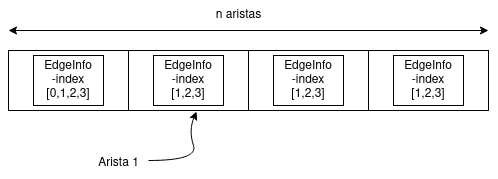
\includegraphics[width=0.75\textwidth]{aristas_v.png} % Include the figure
	\caption{Vector con objetos de aristas}
\end{figure}

De esta manera el vector se pobla al momento de ir formando la lista de adyacencia, y se agregarán los indices vecinos al iterar la lista de adyacencia formando los pares.

\newpage
\section{Experimentación}

\begin{table}[H]
\centering
\begin{tabular}{|l|l|l|l|}
\hline
Kn,n                & Algoritmo   & Llamadas & Tiempo(ns)  \\ \hline
\multirow{2}{*}{10} & Clásica     & 900      & 2870    \\ \cline{2-4} 
                    & Incremental & 36       & 540     \\ \hline
\multirow{2}{*}{20} & Clásica     & 7600     & 23270   \\ \cline{2-4} 
                    & Incremental & 76       & 590     \\ \hline
\multirow{2}{*}{30} & Clásica     & 26100    & 80750   \\ \cline{2-4} 
                    & Incremental & 116      & 1630    \\ \hline
\multirow{2}{*}{40} & Clásica     & 62400    & 173530  \\ \cline{2-4} 
                    & Incremental & 156      & 1609    \\ \hline
\multirow{2}{*}{50} & Clásica     & 122500   & 442890  \\ \cline{2-4} 
                    & Incremental & 196      & 1720    \\ \hline
\multirow{2}{*}{60} & Clásica     & 212400   & 1241580 \\ \cline{2-4} 
                    & Incremental & 236      & 2860    \\ \hline
\multirow{2}{*}{70} & Clásica     & 338100   & 1366080 \\ \cline{2-4} 
& Incremental & 276      & 3010    \\ \hline

\multirow{2}{*}{80} & Clásica     & 505600   & 1644909 \\ \cline{2-4} 
& Incremental & 316      & 2510    \\ \hline
\multirow{2}{*}{90} & Clásica     & 720900   & 2222419 \\ \cline{2-4} 
& Incremental & 356      & 3880    \\ \hline
\multirow{2}{*}{100} & Clásica     & 990000   & 3280289 \\ \cline{2-4} 
& Incremental & 396      & 3020    \\ \hline
\end{tabular}
\end{table}

\begin{figure}[H] % [H] forces the figure to be placed exactly where it appears in the text
	\centering % Horizontally center the figure
	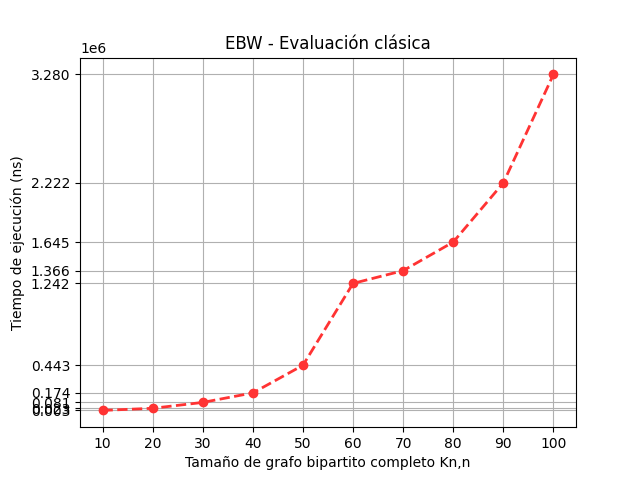
\includegraphics[width=0.65\textwidth]{ebw_clasica.png} % Include the figure
	\caption{Evaluación Secuencial}
\end{figure}

\begin{figure}[H] % [H] forces the figure to be placed exactly where it appears in the text
	\centering % Horizontally center the figure
	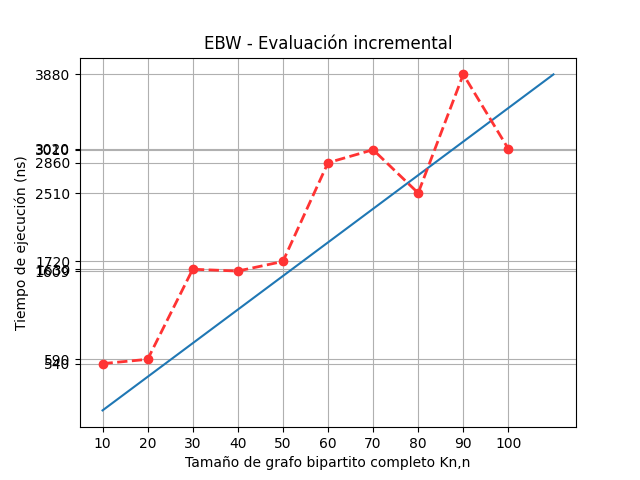
\includegraphics[width=0.65\textwidth]{ebw_incremental.png} % Include the figure
	\caption{Evaluación Incremental}
\end{figure}

%----------------------------------------------------------------------------------------
%	SAMPLE CALCULATION
%----------------------------------------------------------------------------------------

\section{Observaciones}

Considerando los resultados de las graficas déspues de experimentar la corrida con grafos bipartitos completos, el comportamiento es del orden polinomial. Esto es debido al aumento del problema en cada ejecución.\\

En la segunda grafica se observa la tendencia lineal de la evaluación incremental, no obstante no podemos considerar que una es mejor que la otra. Cabe señalar que no atacamos el problema \textbf{max bandwidth} de manera de busca el óptimo y sólo realizamos el intercambio de posiciones evitando recalcular toda la lista de pares de aristas adyacentes. Pero puede ser piedra angular para aplicarlo a una metaheurística de manera de ir encontrando una mejor solución respecto a los objetivos del \textbf{max bandwidth}


\section{Lecciones del curso}

Al cursar el curso de Análisis y diseño de algortimos, logré acercarme al análisis de grafos más allá de lo visto en matemáticas discretas. El poder manipularlo, explorarlo y lograr obtener una herramienta poderosa como lo es una estructura y representación de un grafo. Es bien sabido que varios problemas en nuestra vida cotidiana se pueden llegar a representar con grafos. Tal es así que traté de llevarlo a mis otras materias, así como el empujón que siempre quise tener para comenzar a programar en C++. Salirme de mi zona de confort, y ampliar mis conocimientos en lenguajes que no pasan de moda y altamente portable.\\

Aunque es un hecho que no repartí mi tiempo de forma equitativa entre todas las materias, logré llevar los conocimientos de clase a los demás proyectos como en computo paralelo, desarrollando el proyecto en C++ y cambiando mi paradigma a utilizar algoritmos vistos en clase.\\

Se muy bien que mi desempeño pudó ser mejor y a pesar de los altibajos logré con ayuda del Dr. Eduardo Tello a quién agradezco por sus palabras de aliento cuando imaginaba que mi proyecto de estudiar una Maestria en Ciencias se venía abajo. Eso ya no es un problema para mí, ya que considero que los conocimientos adquiridos este cuatrimestre serán de gran ayuda para el desarrollo de códigos adaptables y modulares cuando me toque regresar a la vida laboral.\\

No espero obtener una buena calificación, pero reconozco el esfuerzo que dedique en la materia con la esperanza de obtener una nota mínima aprobatoria.

\section{Conclusiones}

Como se mencionó en clases, la algorítmica es reconocida como la pieda angular de las ciencias computacionales. El saber de ellas, y aplicarlas es de suma importancia para el desarrollo de códigos limpios.\\

El manejo de abstracciones de clases, las estructuras de datos para generar algoritmos eficientes es de suma importancia. Un ejemplo de ello fué en el presente trabajo donde se logró reducir considerablemente el tiempo de ejecución con simples estructuras aprovechando los ciclos donde se forma la información, para así hacer uso de ellos en pasos posteriores, aunque pueda afectar en el crecimiento espacial, es algo con el que podemos llegar a lidiar. Quitandonos así de tiempos de ejecuciones altos, logrando eficienciar nuestro código.

%----------------------------------------------------------------------------------------
%	BIBLIOGRAPHY
%----------------------------------------------------------------------------------------

\printbibliography % Output the bibliography

%----------------------------------------------------------------------------------------

\end{document}
